

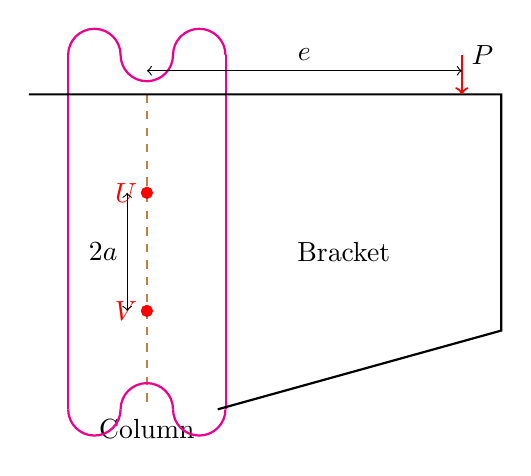
\begin{tikzpicture}

    % Draw the column
    \node[below] at (-0.5, -2) {Column};
\draw[thick,magenta] (-1.5,2.5)--(-1.5,-2);
\draw[thick,magenta] (0.5,2.5)--(0.5,-2);

    % Dashed line for the center of the column
    \draw[dashed, thick, brown] (-0.5,2) -- (-0.5,-2);

    % Draw the bracket
    \draw[thick] (-2,2) -- (4,2) -- (4,-1) -- (0.4,-2);

    % Define the two points
    \coordinate (A) at (-1.5,2.5); % First point
    \coordinate (B) at (0.5,2.5); % Second point

   


 


    \draw[magenta, thick] (-0.834, 2.5) arc[start angle=0, end angle=180, radius=0.333cm];
        \draw[magenta, thick] (-0.834, 2.5) arc[start angle=-180, end angle=0, radius=0.333cm];
    \draw[magenta, thick] (0.498, 2.5) arc[start angle=0, end angle=180, radius=0.333cm];
    
    \draw[magenta, thick] (-1.5, -2) arc[start angle=-180, end angle=0, radius=0.333cm];
        \draw[magenta, thick] (-0.168, -2) arc[start angle=0, end angle=180, radius=0.333cm];
    \draw[magenta, thick] (-0.168, -2) arc[start angle=-180, end angle=0, radius=0.333cm];

     

    % Load P
        \draw[thick, red, ->] (3.5,2.5) -- ++(0,-0.5);

    \node[right] at (3.5,2.5) {$P$};

    % Draw dimension e
    \draw[<->, thin] (-0.5,2.3) -- node[above] {$e$} ++(4,0);

    % Draw points U and V
    \filldraw[red] (-0.5,0.75) circle (2pt) node[left] {$U$};
    \filldraw[red] (-0.5,-0.75) circle (2pt) node[left] {$V$};

 

    % Label for 2a distance
    \draw[<->, thin] (-0.75,0.75) -- node[left] {$2a$} ++(0,-1.5);

    % Label for Bracket
    \node at (2,0) {Bracket};

\end{tikzpicture}

